% *********** Document name and reference:
% Title of document
\renewcommand{\ndoctitle}{MPPNP: The multi-zone parallel frame} 
% Document category acronym 
\renewcommand{\ndocname}{mppnp}                      
% svn dir
\renewcommand{\svndir}{svn://forum.astro.keele.ac.uk/frames/mppnp/DOC}  
% Contributors to this document
\renewcommand{\ndoccontribs}{FH, RH, PD}

%\chapter{\ndoctitle}   % uncomment this if compiled into book in docs directory
\ngtitle{\ndoctitle}     % uncomment this is compiled into chapter wrapper this directory


Document name: \ndocname \\
SVN directory: \svndir\\
%Contributors: \ndoccontribs\\

{  \textbf{Abstract:} \slshape
mppnp is one of the NuGrid frames that uses a physics package and a solver package to post-process multi-zone one-dimensional stellar evolution output.  
}

%\maketitle

%Note that you can mark items that should go into the index
%with \begin{verbatim}\index{items} \end{verbatim}. Reference are
%possible as in \citet{herwig:99a}. The bibtex references are kept in
%ngastro.bib.



\section{Introduction and context}
\index{mppnp} mppnp stands for multi-zone post-processing network
parallel. It is the MPI parallel frame that is used to post-process 1D
stellar evolution model sequences. mppnp uses a farming parallelism. A
master node reads the physics data, input files and USEEPP
files from the SEE library \index{USEEPP}\index{SEE} and sends the
individual mass zones for processing to available slave
nodes. Once these are processed, the results are returned to the master
node, and the idle slave nodes are provided with new work. When all
zones are processed, the master node does a mixing step, handles
grid and I/O functions and proceeds to the next time step.

As with the other frames, mppnp uses the physics and solver
packages to advance a network cell in time. The physics package
provides the nuclear physics input, while the solver package finds the
numerical solution for a given network in one cell for one time step.

mppnp has three grid options. One of them forces calculations on a static grid,
the other, which is a default one, makes mppnp to use a grid from the stellar evolution input. In addition,
there is an option reserved for a future adaptive mesh.

\section{Getting started}
\label{sec:getstarted}

A reorganization of mppnp has recently begun with a main objective to make
it easier and more transparent to use. Therefore, the instructions on how to
compile and run mppnp have changed as of revision 5009 (December 9, 2014).

Here are the new instructions:

\begin{enumerate}
\item 
\texttt{svn update} your nugrid root directory. 
\item
As in the older revisions, set parameter values specific for your machine's OS
and your nugrid installation in the file \texttt{Make.local} in the directory
\texttt{frames/mppnp/CODE}. 
\item
While in the directory \texttt{frames/mppnp},
copy the directory \texttt{RUN\_TEMPLATE} to \texttt{RUN1}
or to a different name of your choice. The copy can be made either
in the same parent directory (\texttt{frames/mppnp}) or at any other place
on your machine.
\item
Go to the new directory that you have just made as a copy of \texttt{RUN\_TEMPLATE}.
If it is located in \texttt{frames/mppnp} then compile an mppnp code right away
by executing the script \texttt{./compile.sh}. If your new directory is
at some other place then, first, specify a path to your nugrid root directory
(i.e. set an appropriate value of the variable \texttt{PPN\_DIR}) in the script
\texttt{config.sh}, then execute \texttt{./compile.sh}.
During the compilation, remarks similar to \texttt{Recommended relationship between 
field width 'W' and the number of\ldots }
may be issued by the compiler. Ignore them, only check that there are no messages about
compilation errors at the very end. You can use the (Linux) command \texttt{ls -l mppnp.exe} 
to make sure that the compilation was successful. It should show
this executable file with the current date and time.
\item
The code compilation script also populates your new \texttt{RUN1} directory with
all the input data files necessary to run \texttt{mppnp}. The only additional thing
you need to do is to open the file \texttt{ppn\_frame.input} and change the path
\texttt{datdir} and \texttt{prefix} that point to the \texttt{see} (stellar evolution and explosion)
\texttt{h5} data files that you are going to post-process. The standard way is to point
to a set of these files on the CADC server, e.g.
\texttt{/tmp/NuGrid/data/set1/set1.1/see\_wind/M2.00Z1.0e-02/M2.00Z0.010},
where \texttt{/tmp/NuGrid} should be replaced with your nugrid vospace mount point
directory name (the instructions on how to mount the VOspace can be found on
the NuGrid website).
\item
The number of CPUs and machines on which mppnp will be running can be changed
in the file \texttt{config.sh}. You don't need to recompile the mppnp code after that.
To start your mppnp post-processing, execute the script \texttt{./run\_me.sh}.
\item
A summary of these instructions can be found in the \texttt{README} file in
your \texttt{RUN1} directory.
\end{enumerate}

\section{Time stepping and cycling}
In the stellar evolution output, mppnp expects an age $t_i$ for cycle
$i$ and a time step $\Delta t_i$, where the structure at age $t_i$ is
the result of integrating (fully implicit) over the time step $\Delta
t_i$ such that $t_{i} = t_{i-1} + \Delta t_i$.  mppnp reads in
density, temperature and mixing coefficient for time $t_i$. To get
the abundances evolved to $t_i$, mppnp needs to advance the abundances
through a fully implicit network over the time step $\Delta t_i$. The resulting
abundances are the abundances at the age $t_i$, and this age needs to be
saved together with the new abundances in the mppnp output file for
cycle $i$.

\section{Grid definition and the adaptive mesh}
In mppnp, a Lagrangian grid point $xm(i)$ is meant to be the location of the
center of the mass cell, which implies that the cell faces are both
$dm_i/2$ away from $xm(i)$.

\section{Building mppnp}
As with all PPN frames, you start with checking out the mppnp frame
from the svn repository.
\begin{quote}
\texttt{ svn co svn://forum.astro.keele.ac.uk:/frames/mppnp}
\end{quote}
This will create a directory \texttt{mppnp} in which you will find
the following directories: \texttt{CODE DOC RUN\_TEMPLATE
  USEEPP}. \texttt{CODE} contains the support
files (Makefile, include files etc) needed to build the code.

\texttt{DOC} contains the documentation for this frame, most
importantly this file. \texttt{RUN\_TEMPLATE} contains templates for
the input files. This directory is completely populated during
the build process when the physics and solver packages are added
to the frame with the input files that go along with it. While
\texttt{RUN\_TEMPLATE} is under svn control, any copy you make to actually
run the code is not.

\texttt{USEEPP} contains some test input data, so that you can run the
code right away. However, any real work will require you to specify
the location and name of the stellar evolution sequence you want to
post-process in the \texttt{ppn\_frame.input} file (Sect.\ \ref{sec:getstarted}).

After the reorganization, the mppnp code is built in a copy of
the directory \texttt{RUN\_TEMPLATE} (for details, see Sect.\ \ref{sec:getstarted}. 
The essential information for building the code is in \texttt{Makefile}. In the top
half of that file, there are parameters that an user can set. The standard
environment for mppnp is a Linux/MacOS platform with OpenMPI and intel
fortran installed. In addition you need to have the USEEPP libraries
and the HDF5 libraries installed. See
\url{http://forum.astro.keele.ac.uk:8080/nugrid/se-library-release}
for details. The latest USEEPP/SE library can of course always be
found on the svn repository.

The only parameter you \emph{have} to set is \texttt{ARCH}, which
stands for architecture. Maybe you recognize the system you are
running on, e.g. on matrix@Keele ARCH=MPIINTEL and any of the 64-bit
systems at UVic can be compiled with ARCH=HELIX. All this is just a
matter of telling the Makefile where \texttt{mpif90} and the
\texttt{se} libraries are installed. Other options are documented in
the \texttt{Makefile}.

The Makefile will first check if a physics and solver source is
available in the CODE directory. If this is not the case, the missing
components will be checked out from svn. This will involve adding the
necessary \texttt{ppn\_physics.input} and \texttt{ppn\_solver.input}
files to the \texttt{RUN\_TEMPLATE} directory. For the physics package
it will involve downloading the \texttt{NPDATA} directory which
contains the raw data for the physics package. Once all the files are
in place the actuall compilation of the executable code will take
place.

Note that the build system allows you to build any previous version of
mppnp, including downloading the physics and solver package that was
current at that previous version of mppnp. Use the parameter
\texttt{REV} in the \texttt{Makefile} for that.

Finally, note that the build process will add a number of directories
to the mppnp directory (on the same level as CODE, DOC etc). None of
these are under svn! So don't make changes to them and expect them to
survive! Also, ppn\_physics.f and ppn\_solver.f in the CODE directory
\emph{don't live there} - so don't change them there, but in the
proper svn places where these packages live on svn.



\section{Running mppnp}
\label{sec:running}

For the new instructions on how to run mppnp, see Sect.\ \ref{sec:getstarted}.

In your \texttt{RUN1} directory have a look at \texttt{README}. You
will find three input files, one for each module:
\texttt{ppn\_frame.input, ppn\_physics.input and ppn\_solver.input}
which are described below (Sect.\ \ref{sec:iofiles}).




\section{Input and run configuration}
\label{sec:iofiles}

Here we describe only the main input file \texttt{ppn\_frame.input}
that is responsible for the frame. The other two input files are
\texttt{ppn\_physics.input} and \texttt{ppn\_solver.input} and are
described in the documentations for the physics and solver packages.

\subsection{Initial composition, start and stop cycle}
\index{ppn\_frame.input} Initialisation of mppnp (r721) is governed by
the following parameters in \texttt{ppn\_frame.input}:
\begin{itemize}
\item \index{modstart} \texttt{modstart:} The stellar evolution cycle
  to start the post-processing. modstart allows you to begin evolution 
  mid hdf5 file. Note that the modstart number that you choose should be 
  contained in the first hdf5 file found in the *.idx file. More 
  information on this *idx file is in section 6.4. 
\item \index{modstop} \texttt{modstop:} The stellar evolution cycle to
  stop the post-processing. modstop allows you to stop stellar evolution
  mid hdf5 file.
\item \index{igrid} \texttt{igrid:} Specifies the post-processing grid 
  (only option 2 is supported at this time (Dec 3, 2009)):\\
\begin{tabularx}{0.9\textwidth}{lX}
  1 & Custom grid as defined in \texttt{subroutine customgrid} that is
  called just before \texttt{subroutine iniabund}. Default custom grid
  is a static grid, but of course anything can be programed into
  \texttt{subroutine customgrid}, as for example done for the
  mppnp-hif/Sakurai version. \\
  2 & stellar evolution grid; use the same grid as the stellar evolution code.  \\
  3 & adaptive mesh refinement \\
   & {\bf Note:} currently, the parameter \texttt{igrid} is hidden in the code. \\
\end{tabularx}
\item \index{iabuini}\texttt{iabuini} How do we initialise the
  post-processing? Fundamentally there are two options. Either we
  continue a previous run, for example in a batch queuing
  environement, in which case we are reading the initial abundance
  from a previous mppnp output. Or we start with some other
  initialisation, a for example at the very beginning of any
  post-processing simulation.\\
\begin{tabularx}{0.9\textwidth}{lX}
1 & Asplund (2005) solar abundance from Urs' file, (../USEEPP/iniab1.0E-02.ppn\_asplund05) \\
2 & solar abundance A\&G89 from gnetw.dat file (../NPDATA/gnetw.dat) \\
3 & fix abundances hardwired in subroutine iniabund  \\
4 & initialise with \texttt{../USEEPP/iniab1.0E-02GN93.ppn} for Set1.1\\
7 & initialise with \texttt{../USEEPP/iniab2.0E-02GN93.ppn} for Set1.2\\
10 & initialise with file specified in parameter \texttt{ini\_file\_name}, the format of the file has to be the same as  \texttt{../USEEPP/iniab1.0E-02GN93.ppn}; can be overloaded with \texttt{xmrmin}, see below. \\
20 & for nova: uses two initial compositions\\
30 & for multi region initialization: Use initial abundances for particular regions of the star, by specifying the number of regions and the mass range for each region.

\end{tabularx}
\item \index{ini\_file\_name}\texttt{ini\_file\_name} Specify name of file
  that contains intial abundance. This name is only recognized if
  \texttt{iabuini=10}. The file is expected to be in
  \texttt{../USEEPP} relative to the run directory.
\item \index{sig\_term\_limit}\texttt{sig\_term\_limit} Sets up an upper limit for diffusion coefficients, similar to and 
by the same reason how and why this is done
 in MESA. A value of \texttt{sig\_term\_limit = 1d+10} is a good choice for most cases, because it results in uniform element
abundance distributions in convective zones, while allowing the code to solve the diffusion equation without numerical problems.
For cases when mixing and nuclear reactions compete in changing element abundances, e.g. for hot-bottom burning,
the sub-time stepping algorithm has to be activated by setting up \texttt{isubmax > 1}. This option is still hidden in the code, 
because the problem of sub-time stepping is not fully solved yet.
\end{itemize}

\subsection{Multi Region Initialization}

For this method, one can divide the star into particular mass regions and then specify an initial abundance file for each of those regions. The input parameters required for this run are the number of regions and the minimum and maximum boundaries of each region, along with their initial abundances. If there are gaps in masses between the regions, then that region is initialized with the \texttt{'background'} initial abundance file. The following example shows how this method was used for post processing a double degenerate WD merger between a CO and an He WD. The parameters specified in \texttt{ppn\_frame.input} are:

\begin{tabularx}{0.9\textwidth}{lX}
\texttt{iabuini=30} \\
\texttt{ini\_file\_name = '../USEEPP/iniab2.0E-02GN93.ppn'} ! The background abundance file \\
\texttt{ini\_file\_name2 = 'co+he\_merger1'}		 ! First file from set of abundance for initializing post processing \\
\end{tabularx}

Three regions are taken into consideration and accordingly there are three \texttt{co+he\_merger}* initial abundance files. The first initial abundance file is \texttt{co+he\_merger1} whose header contains :

\begin{tabularx}{0.9\textwidth}{lX}
$\&$ \texttt{multi\_ini\_abund} \\
\texttt{number\_of\_files = 3}    ! total number of initialization files including this one\\
\texttt{mass\_min = 0.000}       ! initialize with this file in the \\
\texttt{mass\_max = 0.627}       ! region mass\_min $<=$ mass $<$ mass\_max \\
\texttt{name\_next\_file = 'co+he\_merger2'}\\
\end{tabularx}

The above header information has to be appropriately edited and included in the next initial abundance files as well. 

\subsection{Restart capability}
\index{restarts} At cycle intervals \texttt{nprnr} and system time
intervals \texttt{restart} restart dumps are written into
\texttt{*out.h5} output files, see Sect.\,\ref{sec:output}. Whenever
this has successfully happened the corresponding cycle number and the
current packet number will be written into the file
\texttt{last\_restart.out}. Whenever mppnp starts it looks into
\texttt{last\_restart.out}.  The two integers listed in the file reply
to the following 2 questions: 1 $-$ 'From which cycle I want to
start?'; 2 $-$ 'In which packet (hdf5 file) you can find this
cycle?'. You may identify the packet giving the number of the first
cycle in the packet (written also in the name of the packet or HDF5
file).

For a new sequence the file must contain the combination \texttt{0 1}.
\texttt{modstart} and \texttt{iabuini} written in ppn\_frame.input are
considered and give starting informations.  If the first number is
different than zero, the code will ignore \texttt{modstart} and
\texttt{iabuini}, and the code then starts from the restart cycle. At
new start the second integer \texttt{ipacket} has to be set to
\texttt{1} or whatever the new start is supposed to start from.

In case you use \texttt{last\_restart.out} implementation, it is REALLY 
important to following the following steps: 1 $-$ do a cleanall. 
2 $-$ copy a fresh version of the *h5 file that you are using 
to restart from. 3 $-$ copy the original networksetup.txt 
from the RUN directory where the restart *h5 output is coming from in
the working RUN directory.  You can modify rates, swich on and off 
reactions and isotopes, but you CANNOT restart with a different 
networksetup.txt.  This was thought to avoid inconsistencies
(however, it is constraining... still an open issue what it is better to do).
4 $-$ check in the \texttt{last\_restart.out} that
the two numbers \texttt{icycle} and \texttt{ipacket} are still the same that
you want. They are updated during the runs.
This is really important.

The command \texttt{h5ls} is part of the hdf package and should be available on your system. It takes an h5 file as argument and returns the top-level elements in the h5 file, including the restart cycles
\begin{verbatim}
$ h5ls M2.00Z0.010.0009001.out.h5 
A                        Dataset {31}
Z                        Dataset {31}
cycle-10000              Group
cycle-9446               Group
cycle-9500               Group
isomeric_state           Dataset {31}

\end{verbatim}
This will help you to find out which restart cycles are available in a given h5 mppnp output file.

\paragraph{Warning} As of r862 the restart files seem not to be able to withstand multiple restarts from the same file. This may be related to how the SE library overwrites existing cycles, which right now is happening. This needs to be sorted out. As a workaround copy the original h5 output into some tmp directory so that you have a backup should multiple restarts from the same file are requried. 


Support for selem-like initialisation files was deleted in rev.731,
but can be re-introduced any time by checking out a previous version
and copying the code into the current version.
 
\subsection{Sub-time step capability} 
 
MPPNP follows the time steps provided provided by the stellar evolution
input. The timestep size can be reduced by setting a number of sub-time steps
which divide the actual stellar evolution timestep. If activated
the code does not write out all the sub-time steps by default, only in the time steps
provided by the stellar evolution input. Sub-time step information will be added to
the summaryinfo.dat.



\begin{itemize}

\item \texttt{isubmax}\index{isubmax}: Sets the number of sub-time steps MPPNNP will perform.
					  For e.g. isubmax=9 the code will do 10 timesteps instead
					  of 1. If 0, sub-time step capability is turned off.
		
\item \texttt{writeoutsubcycle} \index{writeoutsubcycle}: To write out all sub-time steps
							    into the HDF5 files. last\textunderscore restart.out will
								contain before \texttt{icycle} and \texttt{ipacket}
								the sub-time step cycle number which is necessary
								to restart with the correct cycle number, which differs
								from the stellar evolution cycle to read in next.
\end{itemize}
 
 
 
\subsection{Physics related input}
Most physics input goes into the \texttt{ppn\_physics.input} file. 
\texttt{ppn\_frame.input} only contains \\
\begin{tabularx}{0.9\textwidth}{lX}
  \texttt{t9threshold} & only do nucleosynthesis in cells where T9 is larger \\
  \texttt{ythreshold}  & if abundance lower than ythreshold then abundance = ythreshold
\end{tabularx}




\subsection{Stellar evolution input}
mppnp (r721) needs as input at each timestep the following profiles:
mass, radius, temperature, density, and diffusion coefficient. These
are stored in hdf5 (USEEPP) files. Many hundred and possibly thousand
cycles of input data are typically stored in one USEEPP hdf5 input
file. The parameters in ppn\_frame.input are\\
\begin{tabularx}{0.9\textwidth}{lX}
\texttt{datdir} & character name of path to DATEN directory with
  HPF files
\\
 \texttt{prefix} & prefix for the input hdf5 file and the index
  *.idx file; the *.idx file is the index file of hdf5 files to be
  accessed consecutively. the code will generate an index array to
  know into which hdf5 it has to look to find the thermodynamic input
  for a given cycle. An easy way of making this file is :
  ls -1 *se.h5> filename.idx

\\
\texttt{code\_source} & Unfortunately, we 
do not have the same data available from different stellar evolution 
codes.  Hence, the code parses different stellar evolution data 
differently.  The code\_source option allows the user to specify 
the source of the stellar evolution data:  e.g.\texttt{GVN} for 
Geneva models, \texttt{MES} for MESA or KEPLER (check this) models.  
\end{tabularx}

mppnp allows post-processing of only a small section of the 1D stellar
evolution profile, for example for post-processing only a shell, or a
\cdr-pocket in one interpulse.
\begin{tabularx}{0.9\textwidth}{lX}
\texttt{xmrmin} & The minimum mass radius to post-process from. For
                  nova: if \texttt{xmrmin} $< 0.$ then
                  \texttt{xmrmin}$=0.999\times$\texttt{XMM(1)} where \texttt{XMM(1)} is
                  the outermost mass coordinate, if . 
\\ \texttt{xmrmax} & The maximum
mass radius to post process to.
\end{tabularx}

For the full star use \texttt{xmrmin}$=0$ and
\texttt{xmrmax}$=M_\mem{ini}$.

{\bf Note:} Currently, the parameters \texttt{xmrmin} and \texttt{xmrmax} are hidden in the code.


\section{Output}
\label{sec:output}
Post-processing output is written into hdf5 files of the se type. They
have the ending \texttt{h5}. However, saving
all isotopes at all grid cells for all cycles is likely too much data,
and therefore we store data in the following three ways:
\begin{enumerate}
\item surface data: the surface abundances of all isotopes in the
  network, every cycle, are printed in surf.h5 files along with the shell
  data.  Elemental abundances (in mass fraction )and number abundances
  are also printed.
\item long output: print a full profile for isotopes in the printlist
  (or all of them).  This constitutes the main output for interior
  properties. Usually this would only include the stable and some
  longer-lived unstable species. Note: this output can not be used to
  analyse explosion simulations in which we expect to be even at the
  end of the simulation many species to be in isotopes with shorter
  lifetimes than available in this type of output. For analysis of
  explosion data we use the following:
\item restart: print full profiles of all isotopes to allow for restarts.
  Post-processing runs can resume from the data stored in these
  files. Use this to analyse explosion simulations.
\end{enumerate}
In addition to the isotopes, numerous physical parameters are outputted;
the temperature, density, diffusion coefficient, etc.

There are three variables that implement this:\\
\begin{tabular}{ll}
\texttt{nprnl} & cycle intervals for long ouput \\
\texttt{nprnr} & cycle intervals for restart output\\
\texttt{ioutc} & interval for file creation (in cycles)
\end{tabular}

[Not yet implemented: You can create a printlist file by copying the
isotope list from networksetup.txt to printlist.input and turn the
desired isotopes on using T and F flags]

\paragraph{Old output} If ASCII output is required rather than h5/SE
output, then the old output format can be selected.  This is done by
changing the parameter \texttt{ioutformat} in mppnp.f from 1 to 0 (~ line 2330).
Due to the benefits of using the HDF5 standard for output, the ASCII
output has become dated, but could become useful to some people, for
example, for debugging.\\

Files are given in the format "ABUPPx.DAT" where x is a string
containing the cycle number.  Files are printed out every nprnl cycles.
It contains a self-explanatory header information followed by a table
with the following columns:
\begin{enumerate}
  \item j: shell number \\
  \item xm: Lagrangian mass coordinate\\
  \item t9ppg: temperature \\
  \item rhoppg: density \\
  \item dppg: diffusion coefficient \\
  \item rppg: radius from centre\\
  \item dppgLagr: diffusion coefficient in Lagrangian coordinates\\
  \item NEUT, PROT, H 2, \ldots: abundances of isotopes (mass fractions)
\end{enumerate}
If the parameter \texttt{iprintcsp} in mppnp.f is set to 1 the list
of print species will be taken from \texttt{printlist.input} and
\texttt{printlist.output} will contain an index file with the actually
selected and printed output.  If \texttt{iprintcsp} is set to 0, all
isotopes in the network are printed.

\paragraph{Surface data}
Three abundance variables are printed into the surface yields output:

\begin{enumerate}
   \item yps\_surf: isotope mass fractions
   \item elem\_surf: elemental mass fractions
   \item num\_surf: number abundances
\end{enumerate}
The isotope mass fractions are displayed such that they correspond to the $A$,
$Z$ and Isomer data tables stored in the file.  This is the same style of output
found for the long.h5 and out.h5 files.  Elemental abundances are the sum of the
mass fraction abundances of all isotopes having the same atomic number, $Z$.  
This is always printed in atomic number order (from $Z=0, 1, 2, $\dots to the
maximum value of $Z$ considered in the network), regardless of the isotopes
contained in the network.  For example, if the maximum $Z$ of the network is 26, 
then the surface elements will be:

\begin{verbatim}
elem_surf = (neut, H, He, Li, Be, B, C, N, O, ..., Fe)
\end{verbatim}

This is also true for the number abundances, num\_surf.  Number abundances are
similar to the elemental abundances, but each isotopic mass fraction is divided
by $A$ for that isotope before being summed.

\section{Visualisation}
Visualisation support for all standard plots, including profile plots,
isotopic chart plots, abundance distributions for mass averaged
layers, etc are available via the python module
\index{nugridse.py} \texttt{nugridse.py} that is located in
\texttt{utils/pylib}. Also available are various compilations of
observational data, also presently in the \texttt{utils} top-level svn
directory.

\section{Nova}

Post-processing nova requires accommodating accretion of material that
has a different composition compared to the accreting white
dwarf. Also the white dwarf often has been created using some
\emph{tricks} which means that there is no continuous post-processing
from homogeneous initial composition available. 

The righ thing would be to have a method to trnasform a MESA abundance
profile output into an H5\_restart file by complementing the missing
stable species \emph{somehow}, e.g. with solar scaled abundances. In
the absence of such a method Pavel is following at present a simpler
method. 

\begin{figure}[tbp]
  \centering
   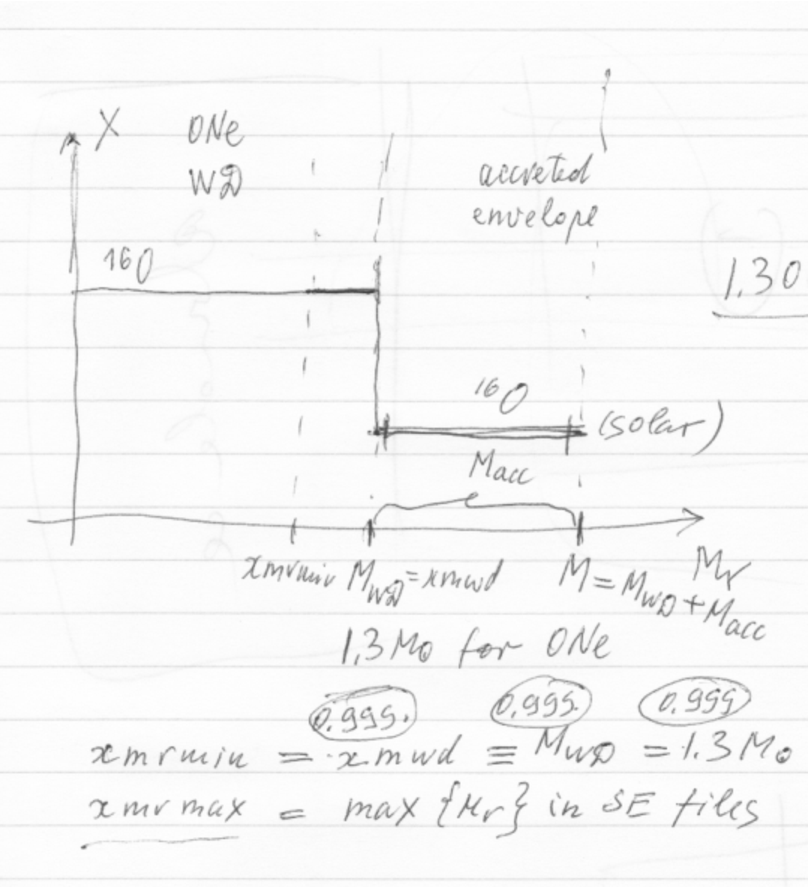
\includegraphics[width=0.75\textwidth]{nova-mppnp.pdf}
   \caption{Schematic view of outer layers of accreting white dwarf,
     demonstrating the meaning of the ppn\_frame.input parameters
    \texttt{xmrmin} and \texttt{xmwd}.[from Pavel Denisenkov]}
   \label{fig:nova_mppnp}
\end{figure}


% --------------------------- end matter ------------------------
\vfill
\section{Document administration}

\subsection{History} 
This document history complements the svn log.

\begin{tabular*}{\textwidth}{lll}
\hline
Authors & yymmdd & Comment \\
\hline
FH & 080616 & generate template \\
RH & ?????? & added IO information \\
FH & 080713 & updated IO, start and restart \\
FH & 090630 & major update and rewrite reflecting new mppnp features \\
MB & 100427 & updated IO information \\
FH & 120224 & updated visualisation info \\
PD & 141209 & update of the instructions on how to build and run the code \\
\hline
\end{tabular*}

\subsection{TODO \& open issues} 
\begin{tabular*}{\textwidth}{lll}
\hline
Requester & yymmdd & Item \\
\hline
FH & 080616 & example request \\
\hline
\end{tabular*}


% --------------- latex template below ---------------------------



%\begin{figure}[htbp]
%   \centering
%%   \includegraphics[width=\textwidth]{layers.jpg} % 
%      \caption{}   \includegraphics[width=0.48\textwidth]{FIGURES/HRD90ms.png}  
%   \includegraphics[width=0.48\textwidth]{FIGURES/HRD150ms.png}  
%
%   \label{fig:one}
%\end{figure}
%
%\begin{equation}
%Y_a = Y_k + \sum_{i \neq k} Y_i
%\end{equation}
%
%{
%%\color{ForestGreen}
%\sffamily 
%  {\center  --------------- \hfill {\bf START: Some special text} \hfill ---------------}\\
%$Y_c$ does not contain ZZZ but we may assign one $Y_n$ to XYZ which is the decay product of the unstable nitrogen isotope JJHJ. %
%
%{\center ---------------  \hfill {\bf END:Some special text} \hfill ---------------}\\
%}

